\chapter{Results}\label{sec:results}

\section{Experiments}\label{sec:experiments}

As already mentioned in the beginning we were interested in two qualities of our system. Most importantly, we wanted to find out what advantages the speed gain with the DVS would provide for quadcopter tracking. An already proven advantage is the opportunity to track active markers.  This is beneficial for searching trackable features as they are easier to identify and thus faster to find. In order to test these performance properties of our algorithm a suitable experimental setup needed to be designed. To measure how fast our system would perform under conditions where convetional cameras tend to perform badly, we planned to test it under real conditions by flying aggressive maneuvers quadcopter while tracking it with the DVS. Furthermore, since the DVS has a much lower resolution than today’s standard CMOS cameras, the accuracy at which pose can be estimated with the DVS needed to be evaluated as well. [Saner] has developed a framework for controlling the ARDrone including the ability to let the drone do a flip, i.e. a 360 degree roll. We decided to use this flip for our aggressive maneuver. As we were only using one camera, that would mean, that the LEDs would lose track somewhere during the flip. Thus we wanted to see for how long the tracking would be lost.


\subsection{Setup}\label{sec:experimentalsetup}

For our setup we used the commercially available ARDrone 2.0 on which we attached our set of four LEDs as well as the microcontroller. Each LED was fixed looking downwards (if one assumes the drone to be in steady flight mode), one under each of the four rotors. All four LEDs where lying on a plane forming a square with 20cm side length. The USB connector available on the drone provided power to the microcontroller and LEDs. For tracking the quadcopter, the DVS was placed on to floor facing upwards.


\subsubsection{Tracking speed comparison}\label{sec:trackingspeedcomparison}

In order to be able to compare the performance of the DVS to a conventional camera, we used the onboard front-looking camera on the quadcopter. The image data was streamed to a computer via network interface, were the parallel tracking and mapping algorithm (PTAM) was employed for pose estimation.


\subsubsection{Pose estimation accuracy}\label{sec:poseaccuracy}

To measure the pose estimation accuracy we needed a reference. For this task we used the OptiTrack from NaturalPoint [link] which is a marker-based optical motion tracking system. It offers millimeter accuracy and was thus a very good approximation to the real positon. Four markers have been applied to the drone in order to make it trackable with the OptiTrack.

\subsubsection{Data recording}\label{sec:datarecording}

Using this setup we did several recordings, where the position data from the OptiTrack, the image data and pose from the drone’s onboard camera, as well as the raw event data from the DVS were recorded.
As the data came from different systems we needed a way to synchronize the measurements afterwards. We decided to use a motion induced cue for synchronization by moving the drone up and down by hand, generating a sinusoid curve in the position data. This was later used for manual time synchronization of the recordings. 
Each recording then started with inducing the cue followed by the drone being remotely piloted to fly over the DVS camera where we would trigger a sideway flip. 


\subsubsection{Difficulties}\label{sec:difficulties}

During the recordings we met a number of unforeseen difficulties. Having attached the LEDs and microcontroller to the drone we found that it had become unstable during flight and hard to control remotely. Although the drone’s motors are powerful enough to pull it upwards fast, which is also necessary in order to do a flip, it had obviously not been designed with additional payload in mind. Another problem of the additional payload was that the drone was not able to output enough power to keep a stable height after the flip. Instead it would usually crashing down on the floor. This meant that a stable reacquisition of the localization with the drone’s internal camera was mostly not possible for a longer time than expected. 
The optical tracking system introduced another challenge into the experiments, since it uses reflection markers for tracking illuminated by high-power infrared spotlights. In the OptiTracks standard setup, the spotlights are pulsed. The DVS is very sensitive to the infrared spectrum and, as we found, the strobing generated a buffer overflow on the DVS as it could not the high amount of events arriving at the same time. Therefore it was very important to deactivate the strobing for all the cameras prior to recording. Also the infrared illumination from the OptiTrack seemed to impede the sensitivity towards our LEDs, although this was not a problem for our experiment setup.


\section{Evaluation}\label{sec:evaluation}

Due to the above difficulties out of 18 executed flips only 6 had feasible data. In the following two paragraphs the measurements of tracking downtime, as well as the pose estimation accuracy will be discussed. Before evaluation the data from the DVS was passed through our algorithm logging the position data output for each recording. 


\subsection{Tracking speed}\label{sec:trackingspeed}

To measure how fast the different systems are able to reacquire tracking we first synchronized the recordings by hand. Since during the recordings the DVS lost track of the LEDs on several occasions, due to them being out of view, the interval during which a flip happened, as well as the time measurements needed to be taken manually. The time for a flip was measured by considering the roll data from the OptiTrack, taking the time between the last measurement before the flip and the first measurement after the flip where the helicopter was in a level orientation to the floor. To measure the onset and offset of losing tracking on the DVS, the last sample before losing track (i.e.  where the interval position samples were considerably higher than the mean sampling rate) and the first sample of reacquiring track (regaining a steady sample rate).  The same was done for the PTAM data. Unfortunately, as previously mentioned, the helicopter usually crashed into the floor after doing a flip. Therefore there often was no stable position data for several seconds. Nevertheless, few single samples with reasonable positioning were recorded before crashing, which were thus taken as the reference. Figure \ref{img:fliptimes} shows a statistical comparison of the time intervals in which the different approaches lost tracking compared to the duration of flips. The red bar indicates the median while the blue box marks the first and third quartile. The whiskers extend to a range of 1.5 times the range between the first and third quartiles. All data points outside this range are considered outliers and are marked with a red plus. Our algorithm lost track during a mean of 0.35 second with a standard deviation of 0.1 seconds. PTAM respectively lost track for a mean of 0.8 seconds with a standard deviation of 0.33 seconds. The average flip took 0.55 seconds with a standard error of 0.15 seconds. One can clearly see that the time where tracking is lost is much shorter with our approach in respect to PTAM. As figure \ref{img:mean_downtime} further illustrates, the downtime for the DVS is shorter than the flip duration. As verified with our recordings the downtime of the DVS corresponds to losing sight of the LED markers because of their emission angle. We reckon that with a suitable configuration of either more markers or cameras, tracking could be maintained during the whole flip. The PTAM data on the other hand shows to lose track for a longer duration than the flip takes. In contrary to the DVS the the camera of the drone loses sight of its tracked features due to blurring in the camera image and thus takes a longer time to recover.

\begin{figure}[h]
     \centering
     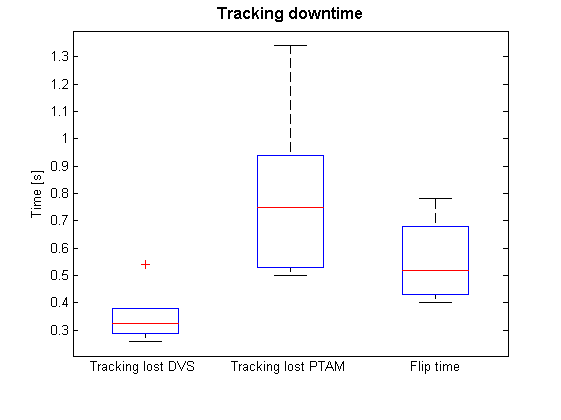
\includegraphics[width=1.0\textwidth]{img/flip_times.png}
     \caption{Statistical plot of measure time interval. The boxplots show the time interval in which tracking is lost for the our algorithm and PTAM compared to the duration of a flip.}
     \label{img:fliptimes}
\end{figure}

\begin{figure}[h]
     \centering
     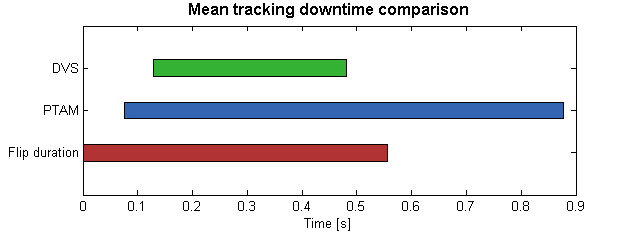
\includegraphics[width=1.0\textwidth]{img/mean_downtime.png}
     \caption{Comparison of the mean tracking downtime intervals. The mean time intervals of both algorithms are compared against the mean flip time on a time line.}
     \label{img:mean_downtime}
\end{figure}

\subsection{Pose estimation}\label{sec:poseestimationeval}

As already mentioned, in order to measure the accuracy of pose estimation from the DVS the OptiTrack data was used as a reference. Apart from synchronizing the measurements in time we also needed to align the different reference frames from the DVS and OptiTrack system first. This was achieved by minimizing function [formula] using the non-linear least squares algorithm from MATLAB. [function explanation] Before doing so the data sets were first brought to the same number of samples with a common time stamps. As the DVS has a lower sampling rate than the OptiTrack the OptiTrack data was resampled by linearly interpolating the translation and rotation. The transformation gained from the least-squares algorithm was then used to align the OptiTrack coordinate system to the one from the DVS. Last, the absolute errors were taken from the translation data. The rotation data, expressed in roll pitch and yaw, again was fitted using the non-linear least squares algorithm from the OptiTrack to the DVS frame. The same analysis was done on the PTAM data in order to compare the two approaches in their accuracy. The mean translation error for the pose estimation over all our recordings was found to be 8.9 cm with a standard error of 12.6 cm. Figure \ref{img:dvs_pose_error_plot} shows the statistical distribution of the pose errors ( for details on the boxplot, please refer to \ref{sec:trackingspeed}). With PTAM a mean translation error of 19 cm with a standard deviation of 12.6 cm was achieved. Our setup shows a clear advantage in accuracy there, as the mean error is twice as low for the translation estimation. As can be seen in [figure] the error from PTAM also has a wider spread than the DVS.

\begin{figure}[h]
     \centering
     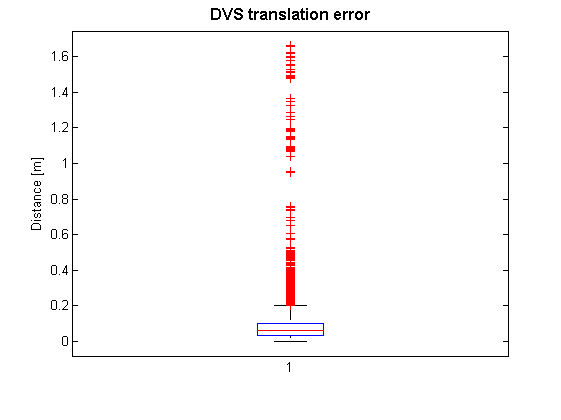
\includegraphics[width=1.0\textwidth]{img/dvs_trans_error_box.png}
     \caption{Statistical plot of the pose estimation error of the DVS in reference to the OptiTrack measurements.}
     \label{img:dvs_pose_error_plot}
\end{figure}

\begin{figure}[h]
     \centering
     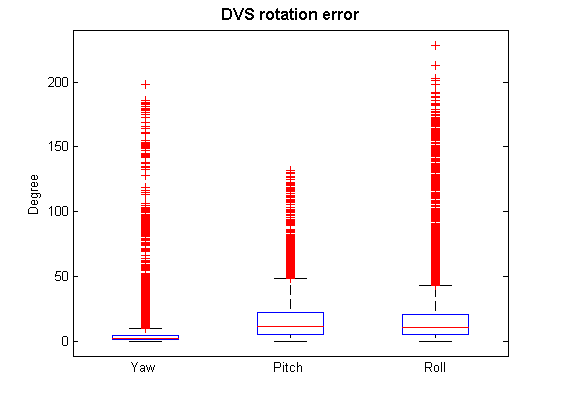
\includegraphics[width=1.0\textwidth]{img/dvs_rot_error_box.png}
     \caption{Statistical plot of the rotation error of the DVS in reference to the OptiTrack measurements.}
     \label{img:dvs_rot_error_plot}
\end{figure}

\begin{figure}[h]
     \centering
     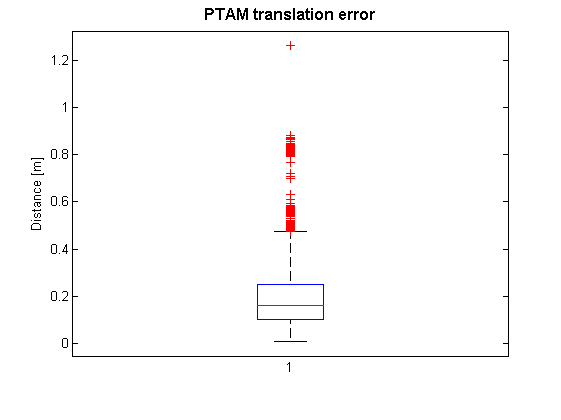
\includegraphics[width=1.0\textwidth]{img/ptam_trans_error_box.png}
     \caption{Statistical plot of the pose estimation error of PTAM in reference to the OptiTrack measurements.}
     \label{img:ptam_pose_error_plot}
\end{figure}

\begin{figure}[h]
     \centering
     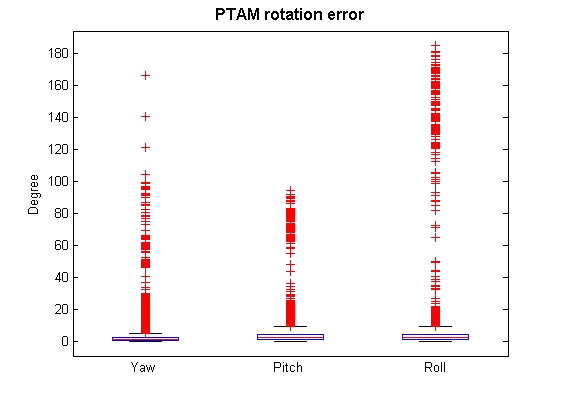
\includegraphics[width=1.0\textwidth]{img/ptam_rot_error_box.png}
     \caption{Statistical plot of the rotation error of PTAM in reference to the OptiTrack measurements.}
     \label{img:ptam_rot_error_plot}
\end{figure}